\documentclass[yuxi]{../template/Report}%方括号内写yuxi即生成预习报告\documentclass[yuxi]{../template/Report}
\settemplatedir{../template/}%设置模板路径

\exname{密立根油滴实验} %实验名称
\extable{} %实验桌号
\instructor{} %指导教师
\class{} %班级
\name{} %姓名
\stuid{} %学号

\nyear{} %年
\nmonth{} %月
\nday{} %日
\nweekday{} %星期几，e.g. \nweekday{三}
\daypart{}%上午/下午，e.g. \daypart{上}

\redate{} %如有实验补做，补做日期
\resitu{} %情况说明：

\begin{document}
\makecover%输出封面

\section{预习报告（10分）}

\subsection{实验综述（5分）}
\subsubsection{实验原理}
实验原理如图所示
\begin{figure}[H]
    \centering
    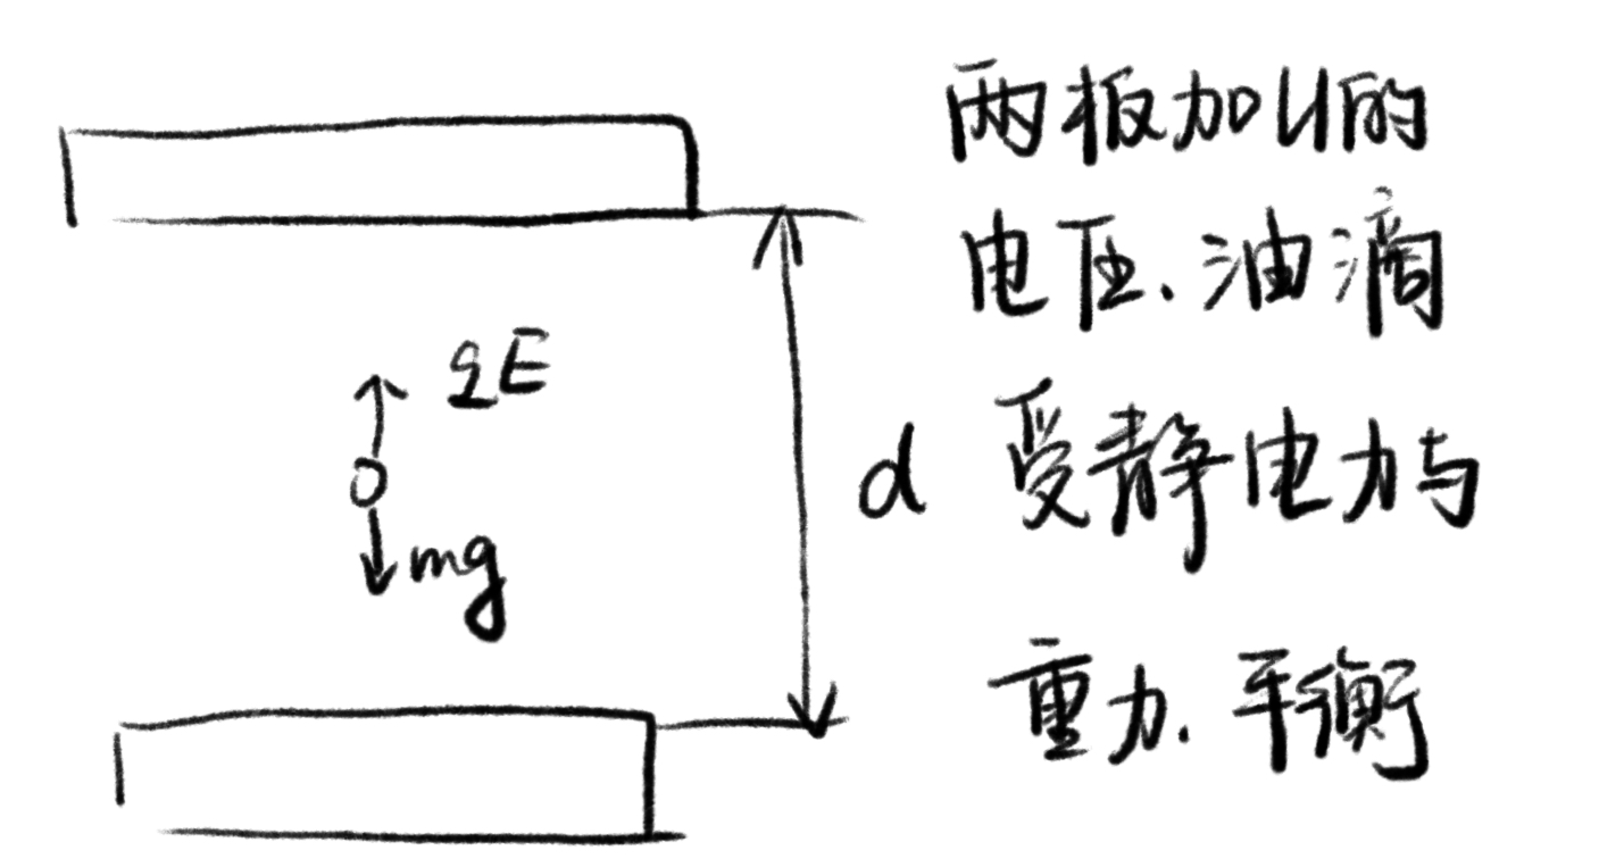
\includegraphics[width=.5\textwidth]{./figures/2/实验原理.pdf}
    \caption{密立根油滴实验原理}
\end{figure}
\begin{enumerate}
    \item \textbf{静态平衡法}

    利用密立根油滴仪的喷雾器将油滴喷入两块相距为 $d$ 的水平放置的平行带电极板间，油滴由于（摩擦）带电，设为 $q$。质量为 $m$，调节极板间电压 $U$ 使油滴平衡，此时根据静电力与重力平衡有：
    \begin{equation}
        mg = qE = q\frac{U}{d} \label{eq:static_balance}
    \end{equation}

    \item \textbf{油滴质量 $m$ 的测定}

    油滴在表面张力作用下，一般呈小球状，设密度为 $\rho$，半径为 $r$，则：
    \begin{equation}
        m = \frac{4}{3}\pi r^3 \rho \label{eq:mass_volume}
    \end{equation}

    考虑空气对油滴的黏滞阻力为 $F$，无电场时油滴（匀速）下降，黏滞阻力 $F$ 与重力 $mg$ 平衡。由斯托克斯定律（$v_g$ 为重力作用下的终端速度）：
    \begin{equation}
        F = 6\pi\eta rv_g = mg \label{eq:stokes_uncorrected}
    \end{equation}

    由 \cref{eq:stokes_uncorrected} 可推导出未修正的 $r$。而 $r \sim 10^{-6} \text{m}$，斯托克斯定律需修正为：
    \begin{equation}
        F = \frac{6\pi\eta rv}{1 + \frac{b}{pr}} \quad (b=6.19 \times 10^{-6} \text{m} \cdot \text{cmHg}, p(\text{cmHg}) \text{为大气压}) \label{eq:stokes_corrected_F}
    \end{equation}

    则修正后的 $mg = F$ 可推导出修正后的半径 $r$：
    \begin{equation}
        r = \sqrt{\frac{9\eta v_g}{2\rho g} \cdot \frac{1}{1 + \frac{b}{pr}}} \label{eq:radius_corrected}
    \end{equation}
    式中 $r$ 可用 \cref{eq:stokes_uncorrected} 式推导出的 $r$ 作近似计算。

    还需测量 $v_g$。设油滴下降 $l$ 用时 $t$，则 $v_g$ 为：
    \begin{equation}
        v_g = \frac{l}{t} \label{eq:vg_def}
    \end{equation}

    \item \textbf{油滴所带电荷量}

    综合上述各式（将 \cref{eq:mass_volume}、\cref{eq:radius_corrected} 和 \cref{eq:vg_def} 代入 \cref{eq:static_balance} 式 $q = mgd/U$），可求得电荷量 $q$ 为：
    \begin{equation}
        q = \frac{18\pi}{\sqrt{2\rho g}} \left[ \frac{\eta v_g}{1+\frac{b}{pr}} \right]^{3/2} \cdot \frac{d}{U} \label{eq:charge_final}
    \end{equation}

    观察发现，总有 $q = ne$，其中 $n$ 为整数，$e$ 是一个不变的定值（基本电荷量）：
    \begin{equation}
        q = ne \quad (n=1, 2, 3, \dots) \label{eq:charge_quantization}
    \end{equation}

\end{enumerate}
\subsubsection{实验内容}

\begin{enumerate}
    \item 仪器调平

    调平仪器，使测量量盘保持水平，从而保证重力方向与电场方向严格平行。

    \item 练习油滴的选择与控制

    \begin{enumerate}
        \item 选择中等大小的油滴:

        油滴太大，则下降速度过快，不利于准确测量时间；油滴太小，则易受布朗运动影响，导致测量误差增大。

        \item 练习控制油滴在视野中的运动，以便随时开始和停止测量。
    \end{enumerate}

    \item 数据测量与获取

    \begin{enumerate}
        \item 将 $K_2$ 开关拨到“平衡”档，调节“平衡电压”旋钮，使视野中的带电油滴在某水平线上静止。记录屏幕显示的平衡电压 $U$ 的大小。

        \item 将 $K_2$ 开关拨到“慢升”档，将该带电油滴移至视野最上缘水平线位置（作为下降起点）。

        \item 将 $K_2$ 开关拨到“0V”档，油滴匀速下降。记录油滴通过一段预定距离 $L$所需的时间 $t$。

        \item 对选定的油滴和新的油滴，重复进行,多次测量，记录数据并填入表格。
    \end{enumerate}

    \item 逐次相减法 确定基本电荷量

    利用上述步骤测量得到的不同油滴所带的电荷量 $q$，通过“逐次相减法”或“最大公约数法”计算出基本电荷量 $e$。并验证所有油滴所带电荷量 $q$ 均是 $e$ 的整数倍。

\end{enumerate}
\subsubsection{实验现象}
\begin{enumerate}
    \item 平行板不加电压时，油滴因重力加速下降，受空气黏滞阻力后匀速；
    \item 加电压使油滴所受重力与静电力平衡，油滴静止;
    \item 改变油滴电荷，平衡电压呈特定值变化。
\end{enumerate}

\subsection{实验重点（3分）}
\begin{enumerate}
    \item 需掌握油滴受力平衡条件，明确重力、静电力、空气黏滞阻力的作用关系，以及电荷量子化的推导逻辑，这是实验数据处理和结果分析的基础；
    \item 测定电子的基本电荷量$e$；
    \item 通过\(e = \frac{q}{n}\)验证电荷的不连续性。
\end{enumerate}

\subsection{实验难点（2分）}
\begin{enumerate}
    \item 难以快速筛选出符合要求的油滴，过大的油滴下降过快，时间测量误差大；过小的油滴易受气流干扰，难以稳定跟踪；
    \item 通过微调电压，确保油滴在 10-20 秒内位置无明显变化，避免因电压调节过度或不足导致误判平衡状态；
    \item 需排除多种干扰因素，如极板电压波动、空气对流等。
\end{enumerate}

\begin{fullreportonly}
\section{原始数据（20分）}
% \begin{figure}[!h]
%     \begin{center}
%         
\includegraphics[width=0.4\textwidth]{./figures/2/data.pdf}
%         \includegraphics[width=0.4\textwidth]{./figures/2/530c184957381481c62600d46fb9f0a4.jpg}
%         \caption{原始数据}
%     \end{center}
% \end{figure}

\section{结果与分析（60分）}
\subsection{数据处理与结果（30分）}
\subsubsection{测量与计算结果}
经过多次测量，记录平衡电压$V$，将开关拨到“0V”挡，选择一段运动计时，记录计时器读数$t$以及下降距离$l$，再应用上述公式：
\[ q = \frac{18\pi}{\sqrt{2\rho g}} \left( \frac{\eta l}{t\left(1 + \frac{b}{pr}\right)} \right)^{\frac{3}{2}} \cdot \frac{d}{U} \]
计算出油滴带电量，得到下表：
\begin{table}[htbp]
  \centering
  \caption{测量所得$V,l,t$及计算所得电荷量$q$}
  \begin{tabular}{@{}ccccccccccc@{}}
    \toprule
    序号 & 1 & 2 & 3 & 4 & 5 & 6 & 7 & 8 & 9 & 10 \\
    \midrule
    \( V(V) \) & 85 & 77 & 78 & 45 & 81 & 44 & 82 & 86 & 30 & 48 \\
    \( l(mm) \) & 1.5 & 1.5 & 1.5 & 1.5 & 1.5 & 1.5 & 1.5 & 1.5 & 1.5 & 1.5 \\
    \( t(s) \) & 21.32 & 25.11 & 25.05 & 23.60 & 15.82 & 25.42 & 15.71 & 21.23 & 32.93 & 20.66 \\
    \( q_i(\times10^{-19}C) \) & 9.55 & 8.15 & 8.07 & 15.3 & 15.9 & 13.9 & 15.9 & 6.42 & 13.6 & 17.7 \\
    \bottomrule
  \end{tabular}
\end{table}

\subsubsection{公约数法计算基本电荷量}
将上述数据中的电荷量升序排列并逐次相减，从而确定各个油滴的基本电荷数$n$，再用$e_i=\frac{q_i}{n}$求得当前油滴的基本电荷量，如下表：
\begin{table}[htbp]
  \centering
  \caption{公约数法计算基本电荷量}
    \begin{tabular}{@{\hspace{1em}}cccccc@{\hspace{1em}}}
    \toprule
    序号 & \( q_i/10^{-19}\text{C} \) & \( q_{i+1}-q_i/10^{-19}\text{C} \) & \( n \)(计算)& \( n \)(取整) & \( e_i \) \\
    \midrule
    1 & 6.42 & 1.65 & 4.01 & 4 & 1.605 \\
    2 & 8.07 & 0.08 & 5.04 & 5 & 1.614 \\
    3 & 8.15 & 1.40 & 5.09 & 5 & 1.630 \\
    4 & 9.55 & 1.05 & 5.97 & 6 & 1.592 \\
    5 & 13.6 & 0.30 & 8.5 & 8 & 1.700 \\
    6 & 13.9 & 1.40 & 8.69 & 9 & 1.544 \\
    7 & 15.3 & 0.60 & 9.56 & 10 & 1.530 \\
    8 & 15.9 & 0.00 & 9.94 & 10 & 1.590 \\
    9 & 15.9 & 1.80 & 10.06 & 11 & 1.590 \\
    10 & 17.7 & — & 11.06 & 11 & 1.609 \\
    \bottomrule
  \end{tabular}
\end{table}
\clearpage
\subsubsection{求相对误差与A类不确定度}
电子电荷的公认值为：\(e_标 = 1.602 \times 10^{-19} \, \text{C}\)

\vspace{2mm}
\textbf{计算测量值的算术平均值\(\bar{e}\):}计算上述数据平均值最终得到
\[\bar{e}=\frac{\sum_{n = 1}^{10}e_i}{10}\approx 1.589 \times 10^{-19} \, \text{C}\]

\textbf{计算相对误差：}将$e_标与\bar{e}$代入相对误差公式：
\[\text{相对误差} = \left| \frac{\bar{e} - e_{\text{标准}}}{e_{\text{标准}}} \right| \times 100\%\]
得到
\[\text{相对误差} = \left| \frac{1.589 - 1.602}{1.602} \right| \times 100\% \approx 0.79\%\]

\vspace{2mm}
\textbf{计算A类不确定度：}A类不确定度公式采用贝塞尔公式，自由度 \( \nu = n-1 = 9 \)：
\[u_A = \sqrt{\frac{1}{n(n-1)} \sum_{i=1}^n (e_i - \bar{e})^2}\]
代入得$u_A \approx 0.013 \times 10^{-19} \, \text{C}$

\vspace{2mm}
最终测量结果可表示为：\(e = (1.589 \pm 0.013) \times 10^{-19} \, \text{C} \quad (\text{相对误差} \approx 0.79\%)\)
\subsection{误差分析（20分）}
\begin{enumerate}
    \item 油滴在实验过程中会逐渐挥发，质量和带电量发生变化，使油滴实际处于动态平衡，难以精准判断静态平衡状态，影响平衡电压的测量；
    \item 油滴并非严格的匀速直线运动，空气阻力与速度的关系及油滴的变速运动过程，会导致下落时间测量存在误差；
    \item 由于人眼观察的局限性，难以精准判断油滴是否完全静止，平衡电压的取值存在误差；
    \item 实验中的空气密度、粘滞系数、重力加速度、大气压等环境参数会随实验条件变化，影响油滴质量、阻力等相关计算。
\end{enumerate}

\subsection{实验探讨（10分）}
在实验操作层面，这是一个对操作技巧要求较高的实验。从喷雾器的使用，到在显微镜下寻找合适的油滴，再到精准调节平衡电压以及测量油滴下落时间，每一个步骤都需要耐心与细心。

\vspace{2mm}
在对实验原理的理解上，我有了更深入的认识。通过实际操作，我更清晰地明白了各个物理量之间的关联，以及公式推导过程中近似处理的意义。

\vspace{2mm}
在数据处理方面，我接触到了 “逐差相减” 等数据处理方法，掌握了一种新的、实用的数据处理思路。

\section{思考题（10分）}
\subsection{在测量油滴匀速下降一段距离$l$所得时间$t$时，应选择哪段$l$最合适？为什么？}

应选择在油滴开始下落（即开关拨到“0V”挡）后，经过了一小段“缓冲”距离之后的区域来测量$l$和$t$。

\textbf{原因如下：}
\begin{enumerate}
    \item \textbf{避免加速阶段：} 油滴在重力、浮力作用下从悬浮开始下落时，会首先经历一个短暂的加速过程。此时其速度尚不稳定。
    \item \textbf{达到终端速度：} 根据斯托克斯定律，空气粘滞阻力与油滴下落的速度成正比，当油滴速度增加到一定值时，空气粘滞阻力与空气浮力之和，会与油滴的重力相平衡。此时油滴所受合外力为零，油滴开始以一个恒定的“终端速度”$v_g$匀速下落。
    \item \textbf{保证测量有效性：} 实验原理中所有关于下落速度的计算（例如 $\eta v_g = mg' $），都要求使用这个恒定的终端速度$v_g = l/t$。如果在油滴刚开始下落、尚未达到匀速的阶段就开始计时，所测得的平均速度将小于其终端速度，导致$t$偏长，这会给后续计算（如油滴半径$r$）带来系统误差。
\end{enumerate}

因此，必须等待油滴运动稳定、进入匀速下落状态后，再开始测量其通过距离$l$的时间$t$。


\subsection{何谓合适的待测油滴？如何选择？}

\textbf{具体标准与选择方法如下：}
\begin{enumerate}
    \item \textbf{亮度适中且清晰：} 在显微镜视野中，应选择那些看起来像一颗明亮、清晰的“小星星”一样的油滴。
    \item \textbf{运动状态稳定：}
        \begin{itemize}
            \item \textbf{避免太小（布朗运动剧烈）：} 如果油滴太小，会受到空气分子碰撞而产生剧烈的布朗运动，在视野中不停地“抖动”，导致无法准确判断其是否静止（平衡）或在匀速运动。
            \item \textbf{避免太大（下落过快）：} 如果油滴太大，其重力远大于电场力或阻力，导致其下落速度$v_g$过快，测量时间$t$过短，这会使得手动计时的相对误差非常大。
        \end{itemize}
    \item \textbf{电荷量适中：} 油滴所带电荷量$q$不能为零（否则无法用电场平衡），但也不宜过大（例如$n>10$）。电荷量过大，会导致用于平衡的电压$V$过低或下落时间$t$过短，

    不利于精确测量。电荷量适中的油滴，其$V$和$t$的数值都处于一个易于精确测量的区间。

    而且受限于测量次数，如果电荷量太大，可能导致逐次相减法得出的元电荷大小为真实值的10倍。
\end{enumerate}
\textbf{选择操作：} 喷入油雾后，打开平衡电场，在视野中搜寻那些亮度适中、受布朗运动干扰较小、能通过调节电压$V$使其稳定悬浮或缓慢上下移动的油滴，作为测量对象。


\subsection{对油滴进行跟踪测量时，有时油滴逐渐变得模糊，为什么？应如何避免在测量途中丢失油滴？}
因为油滴在实验过程中会挥发，质量减小，同时可能受到环境气流等因素影响，导致其与显微镜的对焦状态改变。

\vspace{2mm}
为避免在测量途中丢失油滴，应:
\begin{enumerate}
    \item 尽量选择质量相对较大、挥发较慢的油滴；
    \item 操作时动作轻柔，减少气流扰动；
    \item 密切跟踪油滴的运动，及时微调显微镜焦距，保持油滴始终处于清晰的观察视野中。
\end{enumerate}
\end{fullreportonly}
\insertnotes
\end{document}